\chapter{Test}

\section{Modultest}

\subsection{Software}

\subsubsection{Modultest af Wii-Nunchuck}
På PSoC0 er der software til aflæsning af Wii-Nunchuck input data. Følgende afsnit beskriver test af dette software.

Aflæsning af Wii-Nunchuck sker i to skridt, som begge verificeres ved modul test. Først skal der sendes et \textit{Handshake} fra PSoC0 til Wii-Nunchuck for at initialisere data udveksling, og herefter sker data udveksling hver gang PSoC0 sender en anmodning om det. Disse to skridt modultestes her.

\textbf{Test af Wii-Nunchuck Handshake}

\textbf{Test af data udveksling mellem PSoC0 og Wii-Nunchuck} 

PSoC0 blev programmeret til kontinuert aflæsning af Wii-Nunchuck. For at verificere data udveksling mellem PSoC0 og Wii-Nunchuck blev I2C bussen målt ved brug af Logic Analyzer fra Analog Discovery.

Data udveksling sker i to skridt. Først sender PSoC0 en byte med værdien 0 (0x00 i hexadecimal). Herefter sker den faktiske aflæsning, PSoC0 aflæser Wii-Nunchuck. Begge skridt testes her.

\textbf{Afsendelse af 0x00 byte}

Den første forventede I2C besked er en \textit{0x00} byte fra PSoC0 for at starte en ny aflæsning. På figur \ref{fig:NunchuckWriteValues} ses aflæsningen af I2C bussen på tidspunktet hvor anmodningen til Wii-Nunchuck bliver udført. Dette er en tidslinje læst fra ventre til højre.

\begin{figure}[H]
	\centering
	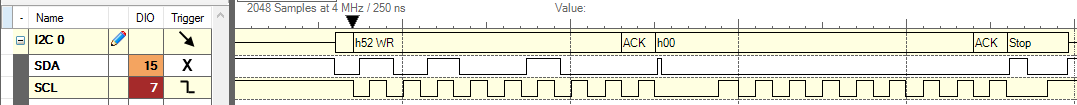
\includegraphics[width=\textwidth]{Test/images/writerequest}
	\caption{}
	\label{fig:NunchuckWriteValues}
\end{figure}

Det kan på figur \ref{fig:NunchuckWriteValues} ses at den første besked der måles er af typen "WR" (Write) til addressen 0x52 (Wii-Nunchuck I2C Slave Addressen). Hertil kommer et tilhørende \textit{ACK} (Acknowledge) fra Wii-Nunchuck. Til sidst sendes dataen Ox00 efterfulgt af at ACK fra Wii-Nunchuck. Til sidst afsluttes I2C transaktionen ved "Stop".

Det kan altså konkluderes at målingen er i overensstemmelse med forventningen om at en 0x00 byte skal sendes til Wii-Nunchuck for opstart af dataudveksling.

\textbf{Aflæsning af Wii-Nunchuck}

Efter vellykket afsendelse af 0x00 byten sker den egentlige aflæsning af Wii-Nunchuk input dataen.

Her forventes en række beskeder indeholdende 

På figur \ref{fig:NunchuckReadValues} ses I2C beskederne der bliver udvekslet mellem PSoC0 og Wii-Nunchuck efter vellykket Wii-Nunchuck Handshake. 

\begin{figure}[H]
	\centering
	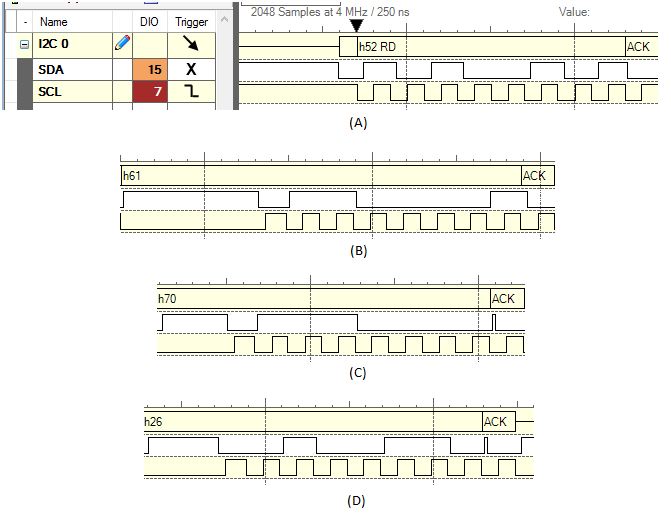
\includegraphics[width=\textwidth]{Test/images/readvaluesEdited.png}
	\caption{Tidslinje af aflæste I2C beskeder af PSoC0 fra Wii-Nunchuck}
	\label{fig:NunchuckReadValues}
\end{figure}

\subsubsection{I2C Protokol}
PSoC0 og PSoC1 kommunikerer over en I2C bus via I2C protokollen beskrevet i afsnit \ref{afsnit:I2CProtokol}. Dette afsnit beskriver test af denne protokol. Følgende test tager udgangspunkt i kommandotypen \textit{NunchuckData} beskrevet i tabel \ref{table:I2CKommandoer}).

\subsubsection{Test af NunchuckData kommandotype} 

Testen blev udført i to dele. I første del måles I2C bussen ved brug af Analog Discovery's Logic Analyzer; for at verificere at den forventede kommandotype bliver overført via bussen. Anden del verificerer at den overførte data er modtaget korrekt via PSoC Creator's debugger.

\subsubsection{NunchuckData kommandotype test del 1}

I testen afsendes, som nævnt i afsnittets indledning, kommandotypen NunchuckData. Som vist i tabel \ref{table:I2CKommandoer} har denne kommandotype ID'et 0xA2, hvor de efterfølgende 3 data bytes indeholder input dataen fra Wii-Nunchuck.

Det forventede resultat af målingen er at første byte er kommandoentypens ID, som har værdien 0x2A. Kommandoens data - de efterfølgende bytes - verificeres først i anden del, disse indgår altså ikke i følgende måling. 

Målingen ses på figur \ref{fig:NunchuckDataCommand}.

\begin{figure}[H]
	\centering
	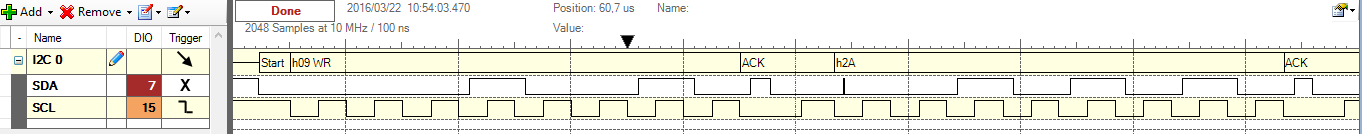
\includegraphics[width=1.2\textwidth]{Test/images/ShowsNunchuckDataCommand.png}
	\caption{Tidslinje af målt I2C kommandotype}
	\label{fig:NunchuckDataCommand}
\end{figure}

Det kan ses på figur \ref{fig:NunchuckDataCommand} at I2C overførslen starter med en I2C \textit{write}, som får et successfuldt acknowledge fra slaven PSoC1. Herefter kan det ses at den næste byte der sendes har værdien 0x2A. Denne byte er kommandoentypens ID, og er altså som forventet 0x2A.

Det kan altså verificeres at kommandoen overføres via I2C bussen. Dataens integritet er dog ikke inkluderet i denne del, og testes i del 2.

\subsubsection{NunchuckData kommandotype test del 2}
For at verificere integriteten af den data der sendes mellem PSoC0 og PSoC1, bruges PSoC Creators indbyggede debugger. Igen er det kommandotypen NunchuckData der sendes mellem de to enheder, hvor de medfølgende data bytes fortolkes.

Testen gennemføres ved at fortolke den modtagne data tre gange, hvor nunchucken er i forskellige tilstande (hvilken retning det analoge stik er trykket) i hver test. Værdierne sammenlignes de forventede standardværdier som ses i tabellen på side 3 i \cite[I2C Interface with Wii Nunchuck]{nunchuck}. Da testene kun er fokuserede på, hvilken retning den analoge pind er presset, er det altså kun receivedDataBuffer[1] (den analoge pinds x-akse) og receivedDataBuffer[2] (den analoge pinds y-akse) der er relevante for testen. Når den analoge pind er presset til venstre, forventes det at receivedDataBuffer[1] er lig \section{TO BE CONTINUED psst. ret pind til stick} 
Disse målinger kan ses på figur \ref{fig:I2CProtocolReadNoInput}, \ref{fig:I2CProtocolReadLeftAnalog} og \ref{fig:I2CProtocolReadUpAnalog}.

\begin{figure}[H]
	\centering
	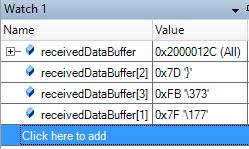
\includegraphics[width=.5\textwidth]{Test/images/I2CProtocolReadNoInput.png}
	\caption{Afmåling af modtager-buffer på PSoC1 efter at have modtaget "NunchuckData" kommando typen. Intet input på Nunchuck'en}
	\label{fig:I2CProtocolReadNoInput}
\end{figure}

\begin{figure}[H]
	\centering
	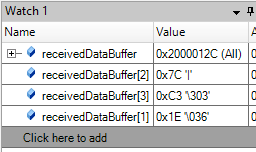
\includegraphics[width=.5\textwidth]{Test/images/I2CProtocolReadLeftAnalog.png}
	\caption{Afmåling af modtager-buffer på PSoC1 efter at have modtaget "NunchuckData" kommando typen. Den analoge pind er presset til venstre på Nunchuck'en}
	\label{fig:I2CProtocolReadLeftAnalog}
\end{figure}

\begin{figure}[H]
	\centering
	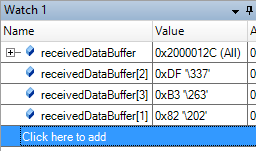
\includegraphics[width=.5\textwidth]{Test/images/I2CProtocolReadUpAnalog.png}
	\caption{Afmåling af modtager-buffer på PSoC1 efter at have modtaget "NunchuckData" kommando typen. Den analoge pind er presset frem på Nunchuck'en}
	\label{fig:I2CProtocolReadUpAnalog}
\end{figure}

\subsection{Hardware}

\section{Integration}

\section{Accepttest}